\section{Multipong} % TODO: Better title?

In this section we will describe how we developed the Multipong application,
focusing on some architectural and implementation choices we made to improve
the game quality.

\subsection{Game description} % TODO: Better title?

Multipong is a tribute to the Pong game, one of the first arcade videogames.
Instead of playing against an AI, there are a single-player mode and a
multiplayer mode.

In the single-player mode the player scores a point each time the paddle hits
the ball, making it bounce upwards until it reaches the top edge and then the
ball falls down again. Clearly, the player loses the game when the paddle misses
the ball.

In the multiplayer mode, several human players connect their devices in order
to form an ad hoc network and then when one of the players hits the ball, it is
transferred to the next player's screen as if their gameboards were joint.
When a player misses the ball, he loses a life and the ball is thrown out
randomly to the next player's screen.
If a player runs out of lives, she will not be able to play for the rest of the
game.

Before starting a multiplayer game a player (called the \textit{host}) creates
a match, allowing other players in his same network to join. Then, when the
game starts, the host will be the initial player.

Since the single-player mode does not involve any significant discussion about
networking and that we did not put any special effort into making the game save
more battery power by optimizing the UI rendering (e.g. we could have improved
the UI rendering performance by using OpenGL), here below we will focus on
discussing the two phases of the multiplayer mode, namely the game formation
and the gameplay.

\subsection{Game formation}

Hereafter we will assume that the players configured correctly a Wi-Fi Direct
ad hoc network with their Android devices, i.e. that they can communicate with
each other within this network.

Since in this phase there are not strong requirements to meet in terms of
real-time information delivering, we decided to use TCP connections until the
game starts. Also, this choice will provide us an element of comparison to the
solution we adopted for gameplay.
Raw data sent over sockets is formatted as JSON objects, so that we are able to
distinguish more easily the requests from one peer to another.

All the design was built having in mind that the topology underneath our system
is an $1:n$ P2P network, so even if the game formation carries out having one
host and several participants, we can not enforce the fact that the host will
also be the GO. Besides this, during the discovery phase only the NGOs will
obtain an address to the GO (and it will be equal to \texttt{192.168.49.1}),
whereas the GO will be notified only of the \textit{presence} of peers, without
obtaining any concrete reference to communicate to them. This means that the
networking logic present in our application have to take into account the fact
that the GO needs to retrieve somehow the IPs of the NGOs.

Before describing the protocols we employed for the game formation phase, we
want to briefly describe how we have implemented data exchange between peers.
Each peer has two threads, respectively for receiving and sending data via the
network. The communication is performed in an asynchronous fashion, so that
messages can be exchanged without blocking on response. However, we implemented
also the semantics for synchronizing on certain operations and we guarantee FIFO
ordering for the data sent out of a device.

In order to create a match among several players, applications on different
devices have to follow a protocol. Firstly, at Wi-Fi P2P discovery time, new
NGOs have to ask to the GO if the application which is running on it is hosting
a game or not by means of a \texttt{ARE\_YOU\_THE\_HOST} message. If so, the
host replies with a \texttt{TELL\_IP} message, otherwise this peer (which is
therefore a participant) replies with a \texttt{KNOWN\_HOSTS} message, in which
the GO lists the hosts it knows.

\begin{figure}[h]
    \centering
    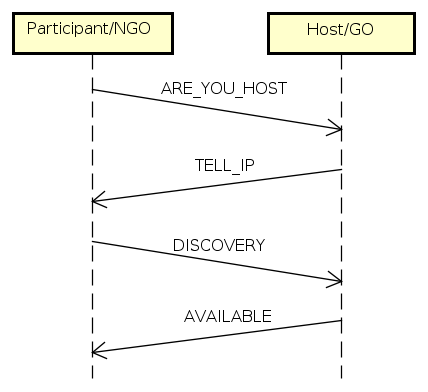
\includegraphics[width=0.30\textwidth]{SequenceDiagram1}
    \caption{Example of communication between a GO-host and an NGO-participant}
    \label{fig:seqDiagram1}
\end{figure}

\begin{figure}[h]
    \centering
    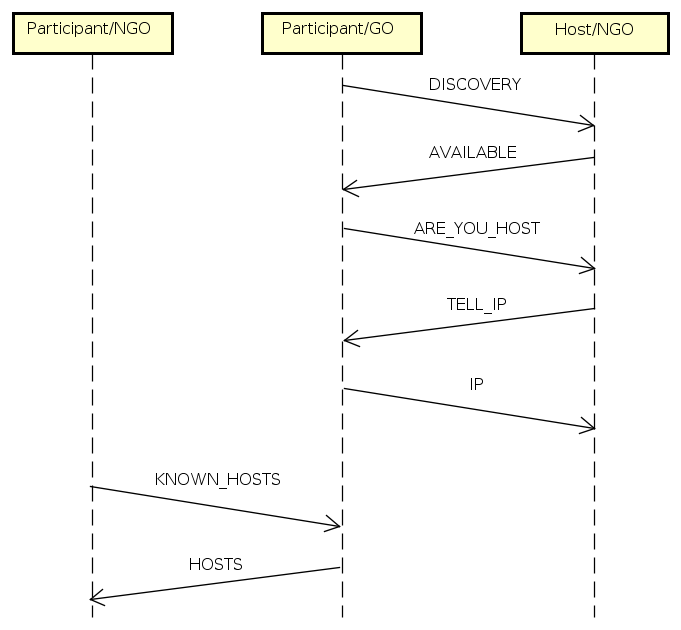
\includegraphics[width=0.30\textwidth]{SequenceDiagram2}
    \caption{Example of communication between an NGO-host, a GO-participant
     and an NGO-participant}
    \label{fig:seqDiagram2}
\end{figure}

Then the participant surely knows the IP of a host (if any) and it is able to
send a \texttt{DISCOVERY} message to the host. This message causes the host to
reply with an \texttt{AVAILABLE} message in which currently joined players are
listed. After this step, the participant can join the message by sending a
\texttt{JOIN} message to the host, receiving back an \texttt{AVAILABLE} message
in which she will be present as a confirmation. Finally, a player can cancel
her subscription by sending a \texttt{CANCEL} message and receiving back an
\texttt{AVAILABLE} message in which she will not be present anymore.

\begin{figure}[h]
    \centering
    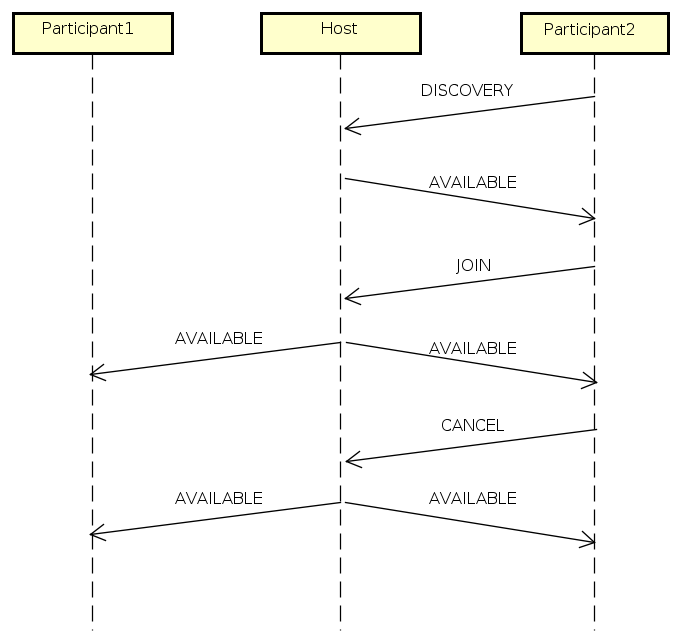
\includegraphics[width=0.30\textwidth]{SequenceDiagram3}
    \caption{Example of communication between a host and two participants,
     in which \emph{Participant1} has just joined the match and
     \emph{Participant2} has not}
    \label{fig:seqDiagram3}
\end{figure}

When a host player sees more than one participant in its match list, she can
decide to start a game, making her Multipong app send a \texttt{STARTING}
message to all of the game participants. Since this is a blocking operation
because it is better not to start the game until all the other players' games
started, the host has to wait for all the messages in its sending queue to be
sent before starting. If some player is unreachable for some reason
during the game starting, she will be excluded by the match as described in
the following subsection.



\subsection{Gameplay}

\begin{figure}[H]
    \centering
    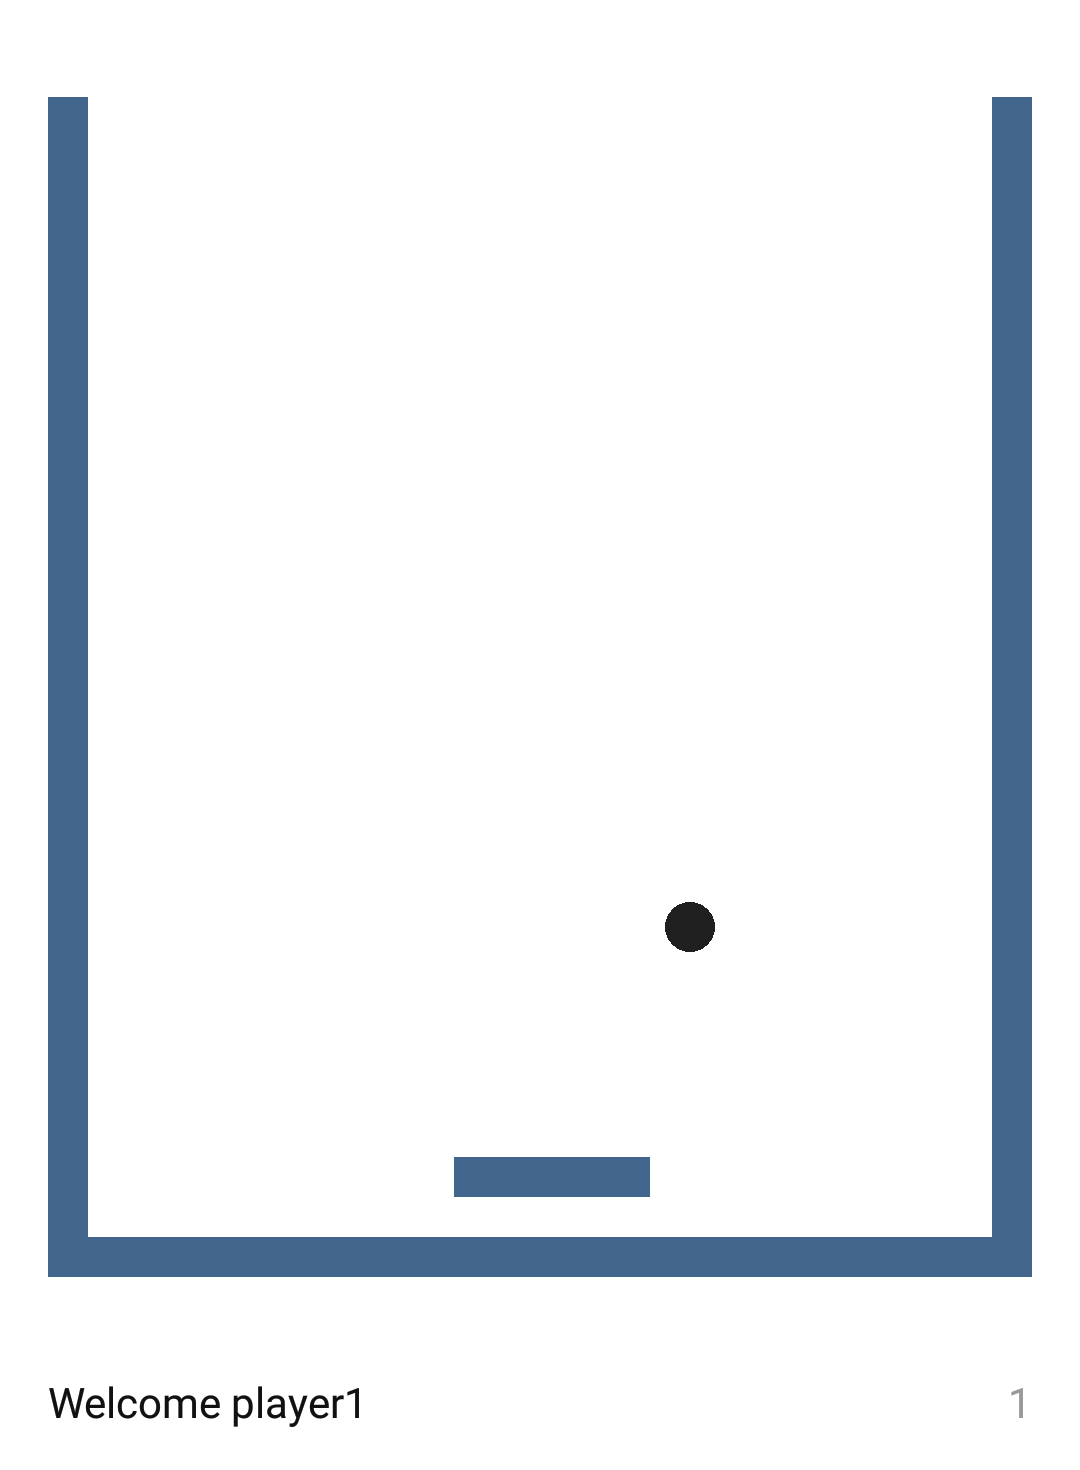
\includegraphics[width=0.23\textwidth]{matchField}
    \caption{Example of match field}
    \label{fig:matchField}
\end{figure}

As anticipated, during the gameplay phase we changed direction regarding the
way we exchange data among peers. In fact, game information messages have to
be delivered very quickly and therefore TCP could not be the best choice for
fast delivery of data. We decided to make peers communicate to each other by
means of an application-level acked UDP transmission: after sending an UDP
packet, a peer waits for a short ACK packet to come back within a short time
frame; if it does not, the peer retries the transmission up to four times in
total.

In this phase of the game we want to have both consistency and low latency, so
that the game can be enjoyable. In order to do so, we designed a two layered
architecture, with one layer that is concerned with coordinating the peers and
the other one that deals with the multiplayer game logic on top of the
coordination layer.

The multiplayer game logic layer has to manage the local state of the game and
part of the global state. Also, when the player hits the ball with the paddle,
it also have to compute the ball exit point from the screen as send this
information to the GO as soon as it is available, so that it can spread this
message to all the active participants of the game. We chose to compute and
send the ball exit position in advance in order to reduce the network latency
perceived by the player.

Just here above we said that a player sends the game information to the GO:
in fact, this entity serves as a global coordinator of the game. We made this
decision so that a reduced amount of traffic has to flow through the network
if only the GO has to care about whether the currently active player is still
live and reachable. Also, the GO is the main entity in the P2P group and this
makes it the most suitable choice for such a role like coordinator.

Clearly, the GO represents a single point of failure during the game phase, but
we want to point out that a network failure such a crash of the coordinator
would make all the ad hoc network collapse. Moreover, recreating a P2P network
is an operation that, at the moment, is quite difficult to carry out in a
short amount of time (and unfortunately things go even worse when done
programmatically). Therefore, we thought that the game of an NGO should end if
it is unable to reach the GO, because restoring the game with the other active
players would be way worse than starting a new one from scratch.

While GO failures are fatal for the game, it copes better with NGOs failures:
in fact, if an NGO happens to look inactive for the GO it is removed from the
game after the GO asked a few times if it is alive or not without getting any
response. In that case, the game continues with the GO telling the other
players that a certain peer is not active anymore.

Game always start from the host device and the queue of players is determined
before the match start. Even if a NGO failure appears the queue of players does
not change, the only difference is that the player with the device that has some
problems is removed from the queue. This strategy is not the only one possible.
In fact we could change the queue of turn of match each turn, but we decided
to maintain always the same for better testability. As a matter of fact that in
this way we could identify the device that presents some problems easily.